\documentclass[]{article}
\usepackage[a4paper, total={6in, 10in}]{geometry}
\usepackage[utf8]{inputenc}
\usepackage{hyperref}
\usepackage{listings}
\usepackage{graphicx}
\usepackage{caption}
\usepackage[backend=biber]{biblatex}
\addbibresource{report.bib}

\begin{document}

\begin{center}
  {\large Data Mining - ID2222}\\
  \vspace{7mm}
  {\huge Homework 3\\[1ex]}
  {\Large  Mining Data Streams }\\
  \vspace{7mm}  
  {André Silva, Jérémy Navarro\\}
  \vspace{4mm}
  {\large November 23, 2020\\}
\end{center}

\section{Overview}

We chose \textit{Python} as the programming language and an \textsc{OOP} approach for the development of the project.\\
We decided to implement the \textit{fully-dynamic} algorithm of the TRIÈST algorithm suite~\cite{triest}.\\
\\
Information about the structure of the project, as well as instructions on how to run it follow:

\begin{lstlisting}[language=bash]
$ unzip homework3.zip
$ cd homework3/
$ python3 main.py
\end{lstlisting}\\
\\
The project is composed by:

\begin{itemize}
    \item \texttt{classes.py}: Contains the classes implementing the chosen algorithm.
    \item \texttt{main.py}: Executable script that uses the algorithm classes on the dataset.
    \item \texttt{facebook\textunderscore combined.txt}: Social circles: Facebook~\cite{facebook}.
\end{itemize}

\section{Classes}

\subsection{FullyDynamic}

The class \texttt{FullyDynamic} takes 1 argument:
\begin{itemize}
    \item \texttt{M}: Number of edges to keep as a sample.
\end{itemize}\\
\\
The class initializes sets and dictionary use to estimate the triangle in the graph streamed.\\
\\
Then, for every new event of the stream, a call to the method \texttt{sample} is necessary. This takes 1 argument, an array representing an edge.\\
\\
Then the algorithm performs as describe in TRIÈST paper~\cite{triest}.

\pagebreak

\section{Results}

\begin{figure}[h!]
    \centering
    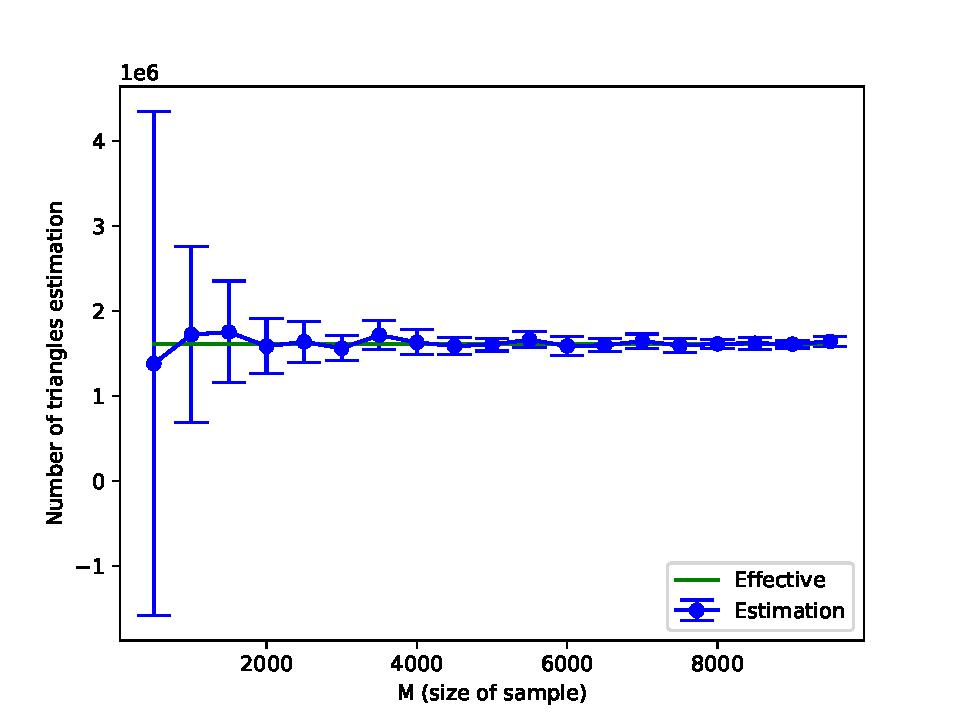
\includegraphics[width=0.72\textwidth,height=\textheight,keepaspectratio]{../experiment.pdf}
    \caption{Estimated number of triangles given a sample size $M$. Points represent means, error bars $2\sigma$, of 20 observations.}
    \label{fig:1}
\end{figure}

\section{\textit{Bonus}}

\subsection{What were the challenges you have faced when implementing the algorithm?}
\label{optimisation}

The main challenges encountered where in the choice of data structures, such that would allow for the algorithm to run efficiently.\\
\\
To represent the graph sample we opted for a set, containing edges, and an adjacency list for each node, stored in a dictionary, which allows us for $O(1)$ access to neighborhoods.\\
\\
To represent the local counters we opted for a dictionary.

\subsection{Can the algorithm be easily parallelized? If yes, how? If not, why? Explain.}

Yes. The main problem with parallelism is concurrent memory access. Indeed, this process can be easily parallelized with a mechanism of mutual exclusion.\\
\\
This being said, we would be losing a lot on efficiency, as our algorithm depends heavily on accessing shared data structures (see \ref{optimisation}), such as the main sample and local, vertex-wise, counters.

\subsection{Does the algorithm work for unbounded graph streams? Explain.}

Yes. As we use random pairing, an extension of reservoir sampling, we only maintain a fixed size sample over the course of the algorithms execution. This is the main advantage of using this type of sampling, as opposed to Bernoulli sampling, where we would keep items with a probability of $p$, making the sample size dependent on the size of the stream.

\subsection{Does the algorithm support edge deletions? If not, what modification would it need? Explain.}

Yes. By using random pairing~\cite{randomsamp}, instead of reservoir sampling, we can handle deletions. This is achieved by making new edge insertion compensate previous deletions.

\printbibliography

\end{document}
